\documentclass[12pt]{article}

%\usepackage{palatino}

\usepackage[utf8]{inputenc}
\usepackage[T1]{fontenc}
\usepackage[sfdefault,scaled=.85, lining]{FiraSans}
\usepackage{newtxsf}
\usepackage[spanish]{babel}
\usepackage{amssymb}
\usepackage{amsmath}
\usepackage{wasysym}
\usepackage[x11names, rgb, html]{xcolor}
\usepackage{graphicx}
\usepackage{caption}
\usepackage{float}
\usepackage{adjustbox}
\usepackage{geometry}
\usepackage{upgreek}
\usepackage[scaled=.85, lining]{FiraMono}
\usepackage[noend]{algpseudocode}
\usepackage{algorithm}
\usepackage[italic]{mathastext}
\usepackage{hyperref}
\usepackage{listingsutf8}

\hypersetup{
  % hidelinks = true,   % Oculta todos los enlaces.
  colorlinks = true,   % Muestra todos los enlaces, sin bordes alrededor.
  linkcolor={black},     % Color de enlaces genéricos
  citecolor={blue!70!black},   % Color de enlaces de referencias
  urlcolor={blue!70!black}     % Color de enlaces de URL
}

\geometry{left=3cm,right=3cm,top=3cm,bottom=3cm,headheight=1cm,headsep=0.5cm}

\setlength{\parindent}{0pt}

%%% COLORES

\definecolor{50}{HTML}{FFEBEE}
\definecolor{100}{HTML}{FFCDD2}
\definecolor{200}{HTML}{EF9A9A}
\definecolor{300}{HTML}{E57373}
\definecolor{400}{HTML}{EF5350}
\definecolor{500}{HTML}{F44336}
\definecolor{600}{HTML}{E53935}
\definecolor{700}{HTML}{D32F2F}
\definecolor{800}{HTML}{C62828}
\definecolor{900}{HTML}{B71C1C}

%% Colores de Solarized

\definecolor{sbase03}{HTML}{002B36}
\definecolor{sbase02}{HTML}{073642}
\definecolor{sbase01}{HTML}{586E75}
\definecolor{sbase00}{HTML}{657B83}
\definecolor{sbase0}{HTML}{839496}
\definecolor{sbase1}{HTML}{93A1A1}
\definecolor{sbase2}{HTML}{EEE8D5}
\definecolor{sbase3}{HTML}{FDF6E3}
\definecolor{syellow}{HTML}{B58900}
\definecolor{sorange}{HTML}{CB4B16}
\definecolor{sred}{HTML}{DC322F}
\definecolor{smagenta}{HTML}{D33682}
\definecolor{sviolet}{HTML}{6C71C4}
\definecolor{sblue}{HTML}{268BD2}
\definecolor{scyan}{HTML}{2AA198}
\definecolor{sgreen}{HTML}{859900}

%% Colores del documento

\definecolor{text}{RGB}{78,78,78}
\definecolor{accent}{RGB}{129, 26, 24}

%%% LISTINGS

%% Tildes

\lstset{
  inputencoding=utf8/latin1
}

\lstset{
  % How/what to match
   sensitive=false,
  % Border (above and below)
  frame=leftline,
  rulecolor=\color{300},
  framerule=2pt,
  % Line number
  numbers=left,
  % Extra margin on line (align with paragraph)
  xleftmargin=\parindent,
  % Put extra space under caption
  belowcaptionskip=1\baselineskip,
  % Colors
  % backgroundcolor=\color{sbase3},
  basicstyle=\footnotesize\ttfamily\color{sbase00},
  keywordstyle=\color{700},
  commentstyle=\color{300},
  stringstyle=\color{500},
  numberstyle=\color{500},
  %identifierstyle=\color{500},
  % Break long lines into multiple lines?
  breaklines=true,
  % Show a character for spaces?
  showstringspaces=false,
  tabsize=2,
  xleftmargin=0.7em,
}

\renewcommand{\lstlistingname}{Código fuente}% Listing -> Algorithm

\title{Metaheurísticas\\ \Large Aprendizaje de Pesos en Características \\ \large Práctica 3: Enfriamiento simulado, búsqueda local reiterada y evolución diferencial}
\author{Antonio Coín Castro \\ XXXXXXXXXXZ \\ XXXXXXXXXX@correo.ugr.es \\ Grupo 1 (M 17:30-19:30)}
\date{\today}

\begin{document}
\maketitle
\tableofcontents

\newpage

\newgeometry{top=3in, left=1.2in, right=1.2in}
\textit{Con el fin de mantener en un único documento toda la información relevante para esta práctica se han incluido en esta memoria las explicaciones y descripciones de los algoritmos que ya se comentaron en la memoria de las prácticas anteriores, así como el análisis de resultados que ya se realizó. Para separar esta información repetida se marcan en {\color{red}rojo} las secciones que no aportan nada nuevo a esta práctica.}
\restoregeometry

\newpage

\section{Descripción del problema}

En todo el desarrollo de las prácticas consideraremos el marco general de un problema de clasificación. Fijado $n \in \mathbb{N}$, un \textit{clasificador} es cualquier función $c: \mathbb{R}^n \to C$, donde $C$ es un conjunto (finito) de clases prefijadas. Consideramos además un \textit{conjunto de entrenamiento} $T \subseteq \mathbb{R}^n$ de elementos ya clasificados: para cada $t \in T$, denotamos $\Gamma(t) \in C$ a su clase, que es conocida.\\

El problema de clasificación consiste en, dado un \textit{conjunto de prueba} $T'\subseteq \mathbb{R}^n$ no observado previamente, encontrar un clasificador $c$ que maximice el número de clases correctamente clasificadas en $T'$, tras haber sido entrenado sobre los elementos de $T$.\\

Uno de los clasificadores más conocidos y más sencillos es el clasificador $k-$NN, que asigna a cada elemento la clase que más se repite entre sus $k$ vecinos más cercanos. En el caso concreto de esta práctica trabajaremos con el clasificador $1-$NN \textbf{con pesos}: a cada elemento le asignamos la clase de su vecino más cercano, pero ponderamos la distancia en función de un vector de pesos $w \in [0,1]^n$.\\

Para el cálculo de la distancia entre dos elementos de $\mathbb{R}^n$ utilizaremos la \textit{distancia euclídea} ponderada por el ya mencionado vector de pesos:

\[
    d_w(t, s) = \sqrt{\sum_{i=1}^n w_i (s_i - t_i)^2}, \quad t, s \in \mathbb{R}^n.
\]
\vspace{.5em}

La idea tras estos pesos es que midan la importancia de cada una de las características que representan las coordenadas de los elementos $n-$dimensionales considerados, asignando más peso en el cálculo de la distancia a aquellas que sean más importantes. El problema de \textbf{aprendizaje de pesos en características} persigue justamente `'aprender'' cuál debe ser el valor de cada peso en una instancia concreta del problema.\\

Para medir la bondad de un clasificador con pesos utilizamos las siguientes métricas:

\begin{itemize}
	\item La \textbf{precisión} (T). Estudiamos cuántos ejemplos del conjunto de prueba se clasifican correctamente, entrenando previamente el clasificador (que utiliza la distancia $d_w$) con el conjunto de entrenamiento.
	\item La \textbf{simplicidad} (R). Un clasificador será más simple si tiene en cuenta un menor número de características. Diremos que una característica $i \in \{1, \dots, n\}$ no se considera en el cálculo de la distancia si su peso asociado $w_i$ es menor que $0.2$.
\end{itemize}

Así, el problema consiste en encontrar un vector de pesos $w \in [0,1]^n$ que maximice la precisión y la simplicidad, es decir, que maximice lo que llamaremos la \textit{función objetivo}:

\[
    F(w) = \alpha T(w) + (1 - \alpha) R(w).
\]

\newpage

\section{Descripción de la aplicación de los algoritmos}

En esta sección se describen los elementos comunes a todos los algoritmos desarrollados, así como los esquemas de representación de datos de entrada y soluciones. Todo el código se ha desarrollado en \verb|C++11|.


\subsection*{{\color{red}Esquemas de representación P1}}

En primer lugar, los datos de entrada se encuentran en la carpeta \verb|DATA|. Consisten en tres conjuntos de datos \textbf{ya normalizados} en formato \verb|csv|, donde cada fila representa un ejemplo con los valores de sus características separados por '\verb|;|' y el último elemento de la fila es su clase.\\

Para representar los datos en el programa se emplea una estructura \verb|Example| que recoge toda la información necesaria: un \verb|vector<double>| con los valores de cada una de las \verb|n| características del ejemplo concreto, así como un \verb|string| que representa su clase o categoría.

\begin{verbatim}
struct Example {
    vector<double> traits;
    string category;
    int n;
};
\end{verbatim}

Cada conjunto de datos se representa entonces por un \verb|vector<Example>|, y se emplea la función \verb|read_csv| para rellenar el vector, que va leyendo los archivos línea a línea.\\

Además, como será necesario hacer particiones de cada conjunto de datos para implementar la técnica de \textit{$K$-fold cross validation}, se proporciona la función \verb|make_partitions| que se encarga de repartir los elementos entre los $K$ conjuntos considerados, respetando la proporción original de clases. La forma de hacer esto es simplemente ir poniendo cada clase de forma cíclica en las particiones, primando el reparto equitativo de clases al reparto equitativo de elementos.\\

Por su parte, la solución es un \verb|vector<double>| del mismo tamaño que el número de categorías consideradas en cada caso. La componente $i-$ésima del vector representa el peso otorgado a la característica $i-$ésima de cada ejemplo del problema.

\subsection*{Esquemas de representación P3}
\label{representacion}
\addcontentsline{toc}{subsection}{\nameref{representacion}}

Añadimos una estructura de datos que representa una solución: un vector de pesos junto con su valor de la función objetivo o \textit{fitness}:

\begin{verbatim}
struct Solution {
    vector<double> w;
    float fitness;
};
\end{verbatim}

Además, para representar una población (para el algoritmo de evolución diferencial) definimos una estructura que engloba varias soluciones, junto con un comparador para ellas, similar al que se empleó para la práctica anterior. El orden definido entre soluciones es el que viene determinado por su \textit{fitness}.

\begin{verbatim}
typedef vector<Solution> Population;

struct SolutionComp {
  bool operator()(const Solution& lhs, const Solution& rhs) {
    return lhs.fitness < rhs.fitness;
  }
} solution_comp;
\end{verbatim}

\subsection*{{\color{red}Operadores comunes P1}}

Todos los algoritmos hacen uso del cálculo de la distancia. Como dijimos, para este cálculo se emplea la distancia euclídea, eventualmente ponderada mediante un vector de pesos. En el caso de que la distancia deseada sea la estándar, se asume que los pesos valen siempre $1$ (en la implementación realmente hay dos funciones separadas, una con pesos y otra sin pesos).

\begin{algorithm}[ht!]
\begin{algorithmic}

\Function{distance\_sq\_weights}{e1, e2, w}
     \State distance = $0$
     \For{i $:=$ $0$ to $n-1$}  \Comment{$n$ es el número de características}
         \If {w[i] $\geq$ 0.2}
            \State distance += w[i] $\ast$ (e2[i] - e1[i]) $\ast$ (e2[i] - e1[i])
         \EndIf
     \EndFor
     \State \Return distance
\EndFunction

\end{algorithmic}
\end{algorithm}

Cabe destacar que en realidad estamos calculando al distancia euclídea al cuadrado, pues solo vamos a utilizarla para comparar. Como la función $f(x)=\sqrt{x}$ es creciente para $x\geq 0$ no hay problema en que hagamos esto, pues se mantiene el orden. De esta forma ahorramos tiempo de cálculo, pues esta función va a ser llamada muchas veces a lo largo del programa.\\

También tenemos la función \verb|classifier_1nn_weights|, que clasifica un ejemplo basándose en la técnica del vecino más cercano. Debemos pasarle también el conjunto de entrenamiento con los ejemplos ya clasificados, y el vector de pesos. De nuevo, si queremos que el clasificador no tenga en cuenta los pesos podemos asumir que son todos $1$, aunque en realidad hay dos funciones separadas.\\

En lo que sigue, para generar números aleatorios reales o enteros utilizamos los tipos predefinidos \verb|uniform_real_distribution| y \verb|uniform_int_distribution|, respectivamente.\\

También se añade una función para \textit{evaluar} un vector de pesos sobre un conjunto de entrenamiento, que devuelve el valor de la función objetivo o \textit{fitness} que obtiene dicho vector. Esta es justo la métrica que vamos a usar para comparar dos vectores de pesos y decidir cuál de ellos es mejor. Es necesario emplear la técnica \textit{leave-one-out}, ya implementada en el clasificador con pesos.

\begin{algorithm}[h]
\begin{algorithmic}

\Function{classifier\_1nn\_weights}{e, training, self, w}
     \State selected = $0$
     \State dmin = $\infty$
     \For{i $:=$ $0$ to $n-1$}  \Comment{$n$ es el número de ejemplos de entrenamiento}
         \If {i $\neq$ self}
            \State dist = distance\_sq\_weights(e, training[i], w)
            \If {dist $<$ dmin}
                \State dmin = dist
                \State selected = i
            \EndIf
         \EndIf
     \EndFor
     \State \Return training[selected].category
\EndFunction

\end{algorithmic}
\end{algorithm}

\begin{algorithm}[ht]
\begin{algorithmic}

\Function{evaluate}{training, w}
    \State classified = $\emptyset$
    \For {i $:=$ $0$ to $n-1$}  \Comment $n$ es el número de ejemplos de entrenamiento
        \State classified.push\_back(classifier\_1nn\_weights(training[i], training, i, w))
    \EndFor
\State \Return objective(class\_rate(classified, training), red\_rate(w))
\EndFunction

\end{algorithmic}
\end{algorithm}

\subsection*{Operadores comunes P3}
\label{op_comunes}
\addcontentsline{toc}{subsection}{\nameref{op_comunes}}

En primer lugar, disponemos de una función \verb|init_solution| que se encarga de generar una solución inicial aleatoria, siguiendo como se pide una distribución uniforme en $[0, 1]$ para los pesos. Esta solución generada se devuelve ya correctamente evaluada.

\begin{algorithm}[h!]
\begin{algorithmic}

\Function{init\_solution}{training, n}
    \State sol = $\emptyset$
    \For {i $:=$ $0$ to $n-1$}  \Comment $n$ es el tamaño del vector de pesos
        \State sol.w[i] = random\_real$(0,1)$
    \EndFor
    \State sol.fitness = evaluate(training, sol.w) 
\State \Return sol
\EndFunction

\end{algorithmic}
\end{algorithm}

También necesitaremos en los tres algoritmos una forma de mutar una solución. Empleamos el esquema de mutación normal descrito en la primera práctica, que consiste en sumarle a una componente del vector de pesos un valor extraído de una distribución normal de media $0$ y desviación típica $\sigma$ (varía según el algoritmo).\\

\begin{algorithm}[ht]
\begin{algorithmic}

\Function{mutate}{w, comp, sigma}
    \State w[comp] += normal$(0, \sigma)$
    \If {w[comp] $< 0$}
        \State w[comp] $= 0$
    \EndIf
    \If {w[comp] $> 1$}
        \State w[comp] $= 1$
    \EndIf
\State \Return w
\EndFunction

\end{algorithmic}
\end{algorithm}

Notamos que al mutar los pesos pueden salirse del intervalo $[0,1]$, por lo que es necesario truncarlos para obtener soluciones que sigan siendo válidas.\\

\subsection*{{\color{red}Función objetivo}}

La función objetivo que queremos maximizar se implementa tal y como se dijo en la descripción del problema, donde el valor $\alpha$ prefijado es de 0.5, dando la misma importancia a la precisión y a la simplicidad.

\begin{verbatim}
objective(class_rate, red_rate) {
  return alpha * class_rate + (1.0 - alpha) * red_rate;
}
\end{verbatim}

Para calcular la tasa de clasificación y de reducción utilizamos otras funciones también muy sencillas. La primera mide el porcentaje de acierto sobre un vector de elementos que el clasificador ha clasificado, y cuya clase real conocemos. La segunda simplemente contabiliza qué porcentaje de los pesos son menores que $0.2$.

\begin{algorithm}[h!]
\begin{algorithmic}

\Function{class\_rate}{classified, test}
    \State correct = $0$
    \For{i $:=$ $0$ to $n-1$}  \Comment{n es el número de ejemplos clasificados}
        \If {classified[i] $==$ test[i].category}
            \State correct++
        \EndIf
    \EndFor
    \State \Return $100.0$ * correct / n
\EndFunction

\end{algorithmic}
\end{algorithm}

\vspace{-1em}

\begin{algorithm}[h!]
\begin{algorithmic}

\Function{red\_rate}{w}
    \State discarded = $0$
    \For{i $:=$ $0$ to $n-1$}  \Comment{n es el tamaño del vector de pesos}
        \If {w[i] $<$ $0.2$}
            \State discarded++
        \EndIf
    \EndFor
    \State \Return $100.0$ * discarded / n
\EndFunction

\end{algorithmic}
\end{algorithm}


\newpage
\section{Descripción de los algoritmos considerados}
En esta sección se describen los algoritmos implementados en esta práctica para el problema del APC. En todos ellos lo que se pretende es rellenar un vector de pesos para maximizar la función objetivo.

\subsection*{Enfriamiento simulado (ES)}
\label{es}
\addcontentsline{toc}{subsection}{\nameref{es}}

El algoritmo de enfriamiento simulado es un algoritmo de búsqueda por trayectorias que persigue paliar uno de los problemas más acusados de la búsqueda local: la caída en óptimos locales. Esto lo hace permitiendo aceptar soluciones peores que la mejor solución actual, aplicando la filosofía de diversificar al principio e intensificar al final.\\

Para llevar a cabo este procedimiento nos basamos en un modelo termodinámico en el que hay una ``temperatura'' figurada que va disminuyendo (enfriando), de forma que a mayor temperatura, mayor probabilidad de aceptación de soluciones peores. Con el aumento de iteraciones disminuye la probabilidad de aceptar soluciones peores que la actual. Así, el algoritmo acepta soluciones mucho peores que la actual al principio de la ejecución (exploración) pero no al final (explotación).\\

Para controlar la probabilidad de aceptación de soluciones utilizamos el modelo de Metrópolis. En este modelo se genera una perturbación (mutación) aleatoria en el sistema y se calculan los cambios de energía resultantes: si hay una caída energética (mejora la solución), el cambio se acepta automáticamente; por el contrario,
si se produce un incremento energético (empeora la solución), el cambio será aceptado con una probabilidad $p = e^{- \Delta f / T}$, donde $\Delta f$ es la diferencia de la función a maximizar sobre las soluciones y $T$ es la temperatura actual del sistema.\\

A la hora de implementar el algoritmo, debemos tener en cuenta que estamos \textbf{maximizando} la función objetivo, por lo que a la hora de calcular la diferencia entre el \textit{fitness} de la solución actual y la mutada debemos ajustar el orden en consecuencia. También modificamos la generación de la temperatura inicial para tener en cuenta este hecho.\\

La \textbf{mutación} de una solución se realiza siguiendo el esquema de mutación normal ya explicado en la sección de operadores comunes. La solución inicial se construye de forma aleatoria.\\

Un último detalle a tener en cuenta es que es posible una solución y su mutación tengan el mismo valor de la función objetivo. En este caso, el modelo de Metrópolis aceptaría siempre la mutación, pero nosotros introducimos una pequeña perturbación en la diferencia para evitar que sea exactamente $0$, y exista la posibilidad de que la mutación sea rechazada.\\

El valor de $M$ pretende representar el número de enfriamientos a realizar para alcanzar el número de iteraciones impuesto, aunque en ocasiones el algoritmo enfría más de la cuenta (debido a la condición extra sobre los éxitos).

\begin{algorithm}[h!]
\begin{algorithmic}

\Function{simulated\_annealing}{training}

\State sol = init\_solution(training, n)  \Comment{n es el número de características}
\State best\_sol = sol
\State $T_0$ = ($0.3$ $\cdot$ ($1 - $ best\_sol.fitness $/$ $100$)) / $- \log(0.3)$
\State $T$ = $T_0$
\State iter = 1
\State successful = 1
\State M = $ 15000$ / $10 \cdot n$

\While {$T_f$ $\geq$ $T$} \Comment{Debe ser $T_0 > T_f$}
    \State $T_f$ = $T$ / 100
\EndWhile

\State $\beta = (T_0 - T_f$) / ($M \cdot T_0 \cdot T_f$)

\While {iter $<$ $15000$ \textit{and} successful $\neq 0$ }
    \State neighbour = 0
    \State successful = 0

    \While {iter $<$ $15000$ \textit{and} neighbour $<$ $10 \cdot n$ \textit{and} successful $<$ $n$}
    \State sol\_mut = mutate(sol, random\_int$(0,1)$, 0.3)
    \State sol\_mut.fitness = evaluate(training, sol\_mut.w)
    \State iter++
    \State neighbour++
    \State $\Delta f$ = sol.fitness - sol\_mut.fitness
    \If {$\Delta f == 0$}
        \State $\Delta f = 0.001$
    \EndIf 
    \If {diff $< 0$ \textit{or} random\_real$(0,1) \leq e^{- \Delta f / T}$}  \Comment{Criterio de Metrópolis}
        \State successful++
        \State sol = sol\_mut
        \If {sol.fitness $>$ best\_sol.fitness}
            \State best\_sol = sol
        \EndIf
    \EndIf
    \EndWhile
    
    \State $T = T$ / $(1 + \beta \cdot T)$  \Comment{Esquema de enfriamiento Cauchy modificado}

\EndWhile

\Return best\_sol.w

\EndFunction
\end{algorithmic}
\end{algorithm}

\subsection*{Búsqueda local reiterada (ILS)}
\label{bl}
\addcontentsline{toc}{subsection}{\nameref{bl}}

La técnica de ILS está basada en la aplicación repetida de un algoritmo de búsqueda local a una solución inicial que se obtiene por mutación brusca de un óptimo local previamente encontrado. En nuestro caso, se utiliza la búsqueda local de la práctica 1, con un máximo de $1000$ iteraciones. El pseudocódigo está en la sección de algoritmos de comparación.\\

Para la mutación de ILS empleamos la misma técnica que venimos usando hasta el momento, pero en vez de sobre una única componente lo hacemos sobre un porcentaje de estas, todas \textbf{distintas}. Además, incrementamos el valor de la desviación típica a $0.4$ para intentar obtener valores más alejados de los originales.\\

Para evitar repetir componentes a mutar utilizamos un \verb|set| llamado \verb|mutated| (que no admite repetidos) en el que insertamos las componentes que ya se han mutado.\\

\begin{algorithm}[h!]
\begin{algorithmic}

\Function{ils}{training}

\State sol = init\_solution(training, n)  \Comment{n es el número de características}
\State s = local\_search(training, s)
\For {i $:=$ 1 to $N-1$}  \Comment {el número de iteraciones es $N=15$}
    \State s\_mut = s
    \State mutated = $\emptyset$
    \For {$j := 0$ to $\lfloor 0.1 \cdot n \rfloor - 1$}  \Comment{Mutación ``brusca''}
        \While {mutated.size() == j}
            \State comp = random\_int$(0, n-1)$
            \State mutated.insert(comp)
        \EndWhile
        
        \State mutate(s\_mut.w, comp, $0.$)
    \EndFor
    
    \State s\_mut.fitness = evaluate(training, s\_mut.w)
    \State s\_mut = local\_search(training, s\_mut)  \Comment{Búsqueda local reiterada}
    
    \If {s\_mut.fitness $>$ s.fitness}  \Comment{Criterio de aceptación}
        \State s = s\_mut
    \EndIf
\EndFor

\State \Return s.w

\EndFunction
\end{algorithmic}
\end{algorithm}

El criterio de aceptación de soluciones es el de la \textbf{mejor solución}. Este criterio favorece la intensificación  o explotación del espacio de búsqueda.

\subsection*{Evolución diferencial (DE)}
\label{ed}
\addcontentsline{toc}{subsection}{\nameref{ed}}

En este caso estamos ante un algoritmo basado en poblaciones que implementa un operador de cruce consistente en generar un vector mutado (según una cierta probabilidad) añadiendo un vector diferencia, escalado y aleatoriamente muestreado, a un vector base aleatoriamente seleccionado de la población actual.\\

Proporcionamos la implementación de dos variantes de este algoritmo, que difieren únicamente en la estrategia de recombinación de vectores. Para el algoritmo \textbf{DE/rand/1} la recombinación sigue la fórmula
$$X^{t+1}_i= X^t_{r_1} + F (X^t_{r_2} - X^t_{r_3}),$$

donde $X^t_i$ es el elemento $i-$ésimo de la población en la generación $t$, $r_1, r_2, r_3$ son índices aleatorios de la población y $F$ es el factor de escala, que en nuestro caso vale $0.5$. Para el algoritmo \textbf{DE/current-to-best/1} la recombinación se puede expresar como
$$X^{t+1}_i= X^t_{i} + F (X^t_{\text{best}} - X^t_{i}) + F(X^t_{r_1} - X^t_{r_2}),$$

donde se ha introducido el término $X^t_{\text{best}}$, que es el mejor elemento de la población actual.\\

Necesitaremos además un operador de selección de padres, que escoja aleatoriamente de la población actual un número determinado de elementos para cruzar. Esta selección se hace sin reemplazamiento, y excluyendo de los candidatos el elemento de la población actual sobre el que se ejecuta el algoritmo general.

\begin{algorithm}[h!]
\begin{algorithmic}

\Function{select\_parents}{pop, num, self}

\State candidates = $\emptyset$  \Comment{es un set sin repetidos}
\For {i $:=0$ to num$-1$}  \Comment {$num$ es el número de padres a seleccionar}
    \While {candidates.size() == i}
        \State index = random\_int$(0, num-1)$
        \If {index $\neq$ self}
            \State candidates.insert(index)
        \EndIf
    \EndWhile
    \State selected.push\_back(pop[index])
\EndFor
\State \Return selected

\EndFunction
\end{algorithmic}
\end{algorithm}

Pasamos ya a describir el algoritmo DE/rand/1. Como en los algoritmos anteriores, la población inicial de soluciones se genera de forma aleatoria. El reemplazamiento es \textit{one-to-one}, es decir, padre e hijo compiten por permanecer en la población.

\begin{algorithm}[h!]
\begin{algorithmic}

\Function{de\_rand}{training}
\State iter = 0
\For {i $:=0$ to $N-1$} \Comment{El tamaño de la población es $N=50$}
    \State pop.push\_back(init\_solution)
    \State iter++
\EndFor

\While {iter $<$ $15000$}
    \For {i $:= 0$ to $N-1$}
        \State parents = select\_parents(pop, 3, i)
        \State chosen = random\_int(0, n - 1) \Comment {n es el número de características}
        \For{k $:= 0$ to $n-1$} 
            \If {k $==$ chosen \textit{or} random\_real$(0,1) \leq CR$} \Comment {$CR = 0.5$}
                \State offspring.w[k] = parents[0].w[k] + F $\cdot$ (parents[1].w[k] - parents[2].w[k])
             \State truncate(offspring.w[k])  \Comment{Truncar a $[0,1]$}.
            \Else
                \State offspring.w[k] = pop[i].w[k]
            \EndIf
        \EndFor
        \State offspring.fitness = evaluate(training, offspring.w)
        \State iter++
        
        \If {offspring.fitness > pop[i].fitness} \Comment{reemplazo}
            \State pop[i] = offspring
        \EndIf
    \EndFor
\EndWhile

\State sort(pop, solution\_comp) \Comment{ordenamos la población de menor a mayor por su \textit{fitness}}

\State \Return pop[N-1].w
\EndFunction
\end{algorithmic}
\end{algorithm}

Observamos que empleamos el esquema de recombinación binomial, mediante el cual primero generamos un índice aleatorio que siempre cambia, y para el resto consideramos una probabilidad de cruce de $0.5$. También debemos tener en cuenta que al aplicar la mutación queremos obtener soluciones válidas (en otro caso truncamos a $[0,1]$).\\

El algoritmo DE/current-to-best/1 es muy similar al ya mostrado, cambiando el esquema de recombinación a la segunda alternativa mencionada anteriormente. En este caso hemos de seguirle la pista al mejor elemento de la población actual.

\begin{algorithm}[h!]
\begin{algorithmic}

\Function{de\_current\_to\_best}{training}
\State iter = 0
\For {i $:=0$ to $N-1$} \Comment{El tamaño de la población es $N=50$}
    \State pop.push\_back(init\_solution)
    \State iter++
\EndFor

\State sort(pop, solution\_comp) \Comment{ordenamos la población de menor a mayor por su \textit{fitness}}
\State current\_best = pop[N-1]

\While {iter $<$ $15000$}
    \For {i $:= 0$ to $N-1$}
        \State parents = select\_parents(pop, 2, i)
        \State chosen = random\_int(0, n - 1) \Comment {n es el número de características}
        \For{k $:= 0$ to $n-1$} 
            \If {k $==$ chosen \textit{or} random\_real$(0,1) \leq CR$} \Comment {$CR = 0.5$}
                \State offspring.w[k] = pop[i].w[k] $+$ F $\cdot$ (current\_best.w[k] - pop[i].w[k]) 
                 \State \hspace{7em} $ +$ F $\cdot$ (parents[0].w[k] - parents[0].w[k])
             \State truncate(offspring.w[k])  \Comment{Truncar a $[0,1]$}.
            \Else
                \State offspring.w[k] = pop[i].w[k]
            \EndIf
        \EndFor
        \State offspring.fitness = evaluate(training, offspring.w)
        \State iter++
        
        \If {offspring.fitness > pop[i].fitness} \Comment{reemplazo}
            \State pop[i] = offspring
        \EndIf
    \EndFor
    \State sort(pop, solution\_comp)
    \State current\_best = pop[N-1]
\EndWhile

\State \Return current\_best.w
\EndFunction
\end{algorithmic}
\end{algorithm}

\newpage
\section{Procedimiento considerado para desarrollar la práctica}

Todo el código de la práctica se ha desarrollado en C++ siguiendo el estándar 2011. Se utiliza la biblioteca \verb|std| y otras bibliotecas auxiliares, pero no se ha hecho uso de ningún \textit{framework} de metaheurísticas.\\

Para todos los procedimientos que implican aleatoreidad se utiliza un generador de números aleatorios común (llamado \verb|generator|), inicializado con una semilla concreta. La semilla por defecto es $2019$, aunque se puede especificar otra mediante línea de comandos. La evaluación de todos los algoritmos considerados se realiza mediante la función \verb|run_p3|, que también se encarga de recoger las estadísticas oportunas.\\

Se proporciona un makefile para compilar los archivos y generar un ejecutable (con optimización \verb|-O3|), mediante la orden \verb|make p3|. A la hora de ejecutarlo hay dos opciones:

\begin{itemize}
    \item Pasarle como parámetro una semilla para el generador aleatorio, y a continuación una lista de archivos sobre los que ejecutar los algoritmos (ruta relativa).
    \item Ejecutarlo sin argumentos. En este caso, utiliza la semilla por defecto y ejecuta los algoritmos sobre los tres conjuntos de datos de la carpeta \verb|DATA|.
\end{itemize}

El código está disponible en la carpeta \verb|FUENTES|, y consta de los siguientes módulos:

\begin{itemize}
	\item \verb|p3.cpp| Contiene la implementación de los algoritmos, y las funciones necesarias para ejecutarlos.
	\item \verb|timer| Módulo para medir tiempos en UNIX.
	\item \verb|util| Se trata de funciones auxiliares para el preprocesamiento de los archivos de datos, el cálculo de la distancia, etc.
\end{itemize}

Al compilar se genera un único ejecutable en la carpeta \verb|BIN| de nombre \verb|p3|.\\

Todas las ejecuciones se han realizado en un máquina con sistema operativo \verb|Linux| y procesador Intel Core i5-7200U @ 2.5GHz.

\newpage
\section{Algoritmos de comparación}

Para comparar las metaheurísticas implementadas en esta práctica usaremos los algoritmos implementados en la práctica 1, a saber: el clasificador $1-$NN sin pesos, el algoritmo RELIEF y la búsqueda local. También compararemos en ciertos casos con los algoritmos genéticos y meméticos de la práctica 2.

\subsection*{{\color{red} Clasificador $\mathbf{1}$-NN sin pesos}}

Ya se ha descrito en la sección de operadores comunes (podemos considerar que es un clasificador con pesos, donde todos los pesos valen $1$).

\subsection*{{\color{red} Algoritmo \textit{greedy} RELIEF}}

Este es un algoritmo voraz muy sencillo, que servirá como caso base para comparar las diferentes metaheurísticas desarrolladas. Se trata de buscar, para cada ejemplo, su amigo (misma clase) y su enemigo (distinta clase) más cercano. Después, componente a componente se suma al vector de pesos la distancia a su enemigo, y se resta la distancia a su amigo.\\

En este proceso es posible que los pesos se salgan del intervalo $[0,1]$, por lo que al finalizar es necesario normalizarlos. Además, no debemos olvidar que el algoritmo comienza con el vector de pesos relleno de $0$s. Disponemos para ello de una función \verb|init_vector| que se encarga de darle un valor inicial de $0$ a todas las componentes del vector de pesos.\\

Separamos la función que se encarga de buscar los amigos y enemigos más cercanos, teniendo en cuenta que el amigo más cercano no puede ser el propio ejemplo.

\begin{algorithm}[h]
\begin{algorithmic}

\Function{nearest\_example}{training, e, self}
     \State dmin\_friend = $\infty$
     \State dmin\_enemy = $\infty$
     \For{i $:=$ $0$ to $n-1$}  \Comment{n es el número de ejemplos de entrenamiento}
         \If {i $\neq$ self}
            \State dist = distance\_sq(e, training[i])
            \If {training[i].category $!=$ e.category \textit{and} dist < dmin\_enemy}
                  \State n\_enemy = i
                  \State dmin\_enemy = dist
            \ElsIf {training[i].category == e.category \textit{and} dist < dmin\_friend)}
                  \State n\_friend = i
                  \State dmin\_friend = dist
            \EndIf
          \EndIf
       \EndFor
   \State \Return n\_enemy, n\_friend
\EndFunction

\end{algorithmic}
\end{algorithm}

El algoritmo RELIEF se detalla ya en la página siguiente.
\newpage

\begin{algorithm}[h!]
\begin{algorithmic}

\Function{relief}{training}
     \State w = init\_vector()
     \For{i $:=$ $0$ to $n-1$}  \Comment{n es el número de ejemplos de entrenamiento}
         \State n\_enemy, n\_friend = nearest\_example(training, training[i], i)
         \For{j $:=$ $0$ to $m - 1$}  \Comment {m es el tamaño del vector de pesos}
            \State w[j] = w[j] + $|$training[i].traits[j] - training[n\_enemy].traits[j]$|$
            \State \hspace{2.5em} $-$ $|$training[i].traits[j] - training[n\_friend].traits[j]$|$

         \EndFor
      \EndFor
      \State max = max(w)
      \For {j $:=$ $0$ to $m-1$}  \Comment{normalizamos los pesos}
        \If {w[j] $<$ 0}
            \State w[j] = 0
        \Else
            \State w[j] = w[j] / max
        \EndIf
      \EndFor
\State \Return w
\EndFunction

\end{algorithmic}
\end{algorithm}


\subsection*{{\color{red} Búsqueda local}}

Empleamos la técnica de búsqueda local del \textbf{primer mejor} para rellenar el vector de pesos. La idea es mutar en cada iteración una componente aleatoria y \textbf{distinta} del vector de pesos, sumándole un valor extraído de una normal de media $0$ y desviación típica $\sigma = 0.3$. Si tras esta mutación se mejora la función objetivo, nos quedamos con este nuevo vector, y si no lo desechamos. Si algún peso se sale del intervalo $[0,1]$ tras la mutación, directamente lo truncamos a $0$ ó a $1$.\\

A la hora de escoger qué componente vamos a mutar, tenemos un vector de índices del mismo tamaño que el vector de pesos, que barajamos de forma aleatoria y recorremos secuencialmente. Si llegamos al final, volvemos a barajarlo para seguir generando nuevas soluciones. \\

Para escoger el valor con el que se muta cada componente utilizamos esta vez el tipo predefinido \verb|normal_distribution<double>|. Para determinar si una mutación mejora, utilizamos como métrica el valor de la función objetivo, tomando la tasa de clasificación sobre el propio conjunto de entrenamiento (\textit{leave-one-out}). \\

Hemos adaptado ligeramente este algoritmo con respecto al implementado en la práctica 1, para que acepte como parámetro un elemento de tipo \verb|Solution|, que hace las veces de solución inicial.\\

\vspace{20em}

\begin{algorithm}[ht!]
\begin{algorithmic}

\Function{local\_search}{training, s}

\State index = initialize() \Comment{vector de índices de 0 a $n$}

\State best\_fitness = evaluate(training, w)

  \While {iter $<$ MAX\_ITER \textit{and} neighbour $<$ n * MAX\_NEIGHBOUR\_PER\_TRAIT}
    \State comp = index[iter $\%$ n] \Comment{n es el número de características}
    \State s\_mut = s
    \State mutate(s\_mut, comp, $0.3$)
    \State s\_mut.fitness = evaluate(training, s\_mut.w)
    \State iter++

    \If {s\_mut.fitness $>$ best\_fitness}
      \State neighbour = $0$
      \State s = s\_mut
      \State best\_fitness = s\_mut.fitness
      \State improvement = true

    \Else
      \State neighbour++
    \EndIf

    \If {iter $\%$ $n == 0$ \textit{or} improvement}
      \State shuffle(index.begin(), index.end(), gen)
      \State improvement = false
    \EndIf
  \EndWhile

\State \Return w
\EndFunction

\end{algorithmic}
\end{algorithm}

Notamos que detenemos la búsqueda cuando llegamos al máximo de iteraciones, o cuando generamos un número de vecinos (dependiente del número de características) sin mejorar la función objetivo.

\subsection*{{\color{red} Algoritmos genéticos y meméticos}}

Aunque no se vuelven a describir en esta memoria los algoritmos genéticos y meméticos implementados en la práctica anterior, se mantienen en la tabla global de resultados para compararlos con los algoritmos de evolución diferencial, que también son algoritmos basados en poblaciones.

\newpage
\section{Resultados}

\subsection*{Descripción de los casos del problema}
\label{casos}
\addcontentsline{toc}{subsection}{\nameref{casos}}

Se consideran tres conjuntos de datos sobre los que ejecutar los algoritmos:

\begin{itemize}
	\item \textbf{Colposcopy.} La colposcopia es un procedimiento ginecológico que
consiste en la exploración del cuello uterino. Consta de 287 ejemplos, 62 atributos reales y dos clases: positivo o negativo.
    \item \textbf{Ionosphere.} Datos de radar recogidos por un sistema en Goose Bay, Labrador. Consta de 351 ejemplos, 34 atributos y dos clases: retornos buenos (g) y malos (b).
    \item \textbf{Texture.} El objetivo de este conjunto de datos es distinguir entre 11
texturas diferentes. Consta de 550 ejemplos, 40 atributos y 11 clases (tipos de textura).
\end{itemize}

\subsection*{Resultados obtenidos}
\label{resultados}
\addcontentsline{toc}{subsection}{\nameref{resultados}}

A continuación se muestran las tablas de unos resultados obtenidos para cada uno de los algoritmos. El orden de las columnas es siempre el mismo: primero \textit{colposcopy}, después \textit{ionosphere}, y por último \textit{texture}. La semilla utilizada es la semilla por defecto: $2019$.\\

Para cada conjunto de datos se muestra una tabla con cada una de las 5 ejecuciones realizadas, de acuerdo a la técnica $5-$\textit{fold cross validation}. En cada una de ellas se muestran los valores de la tasa de clasificación (Clas), tasa de reducción (Red), función objetivo (Agr) y tiempo de ejecución (T) \textbf{en segundos}. Además, se muestra finalmente una tabla global con los resultados medios de cada conjunto de datos para todos los algoritmos. Esta información también se recoge en la última fila de las tablas de cada algoritmo.\\

{\color{red}\textbf{Clasificador $\boldsymbol{1-}$NN sin pesos}}

\begin{table}[ht!]
\begin{tabular}{ccccc|cccc|cccc}
\centering
 & \multicolumn{4}{c}{\textit{Colposcopy}} & \multicolumn{4}{c}{\textit{Ionosphere}} & \multicolumn{4}{c}{\textit{Texture}} \\ \hline
\textbf{Nº} & \textbf{Clas} & \textbf{Red} & \textbf{Agr} & \textbf{T} & \textbf{Clas} & \textbf{Red} & \textbf{Agr} & \textbf{T} & \textbf{Clas} & \textbf{Red} & \textbf{Agr} & \textbf{T} \\ \hline
1 & 69.49 & 0.00 & 34.75 & 0.001 & 88.73 & 0.00 & 44.37 & 0.001 & 93.64 & 0.00 & 46.82 & 0.002\\
2 & 75.44 & 0.00 & 37.72 & 0.001 & 90.00 & 0.00 & 45.00 & 0.001 & 96.36 & 0.00 & 48.18 & 0.002\\
3 & 70.18 & 0.00 & 35.09 & 0.001 & 91.43 & 0.00 & 45.71 & 0.001 & 92.73 & 0.00 & 46.36 & 0.002\\
4 & 77.19 & 0.00 & 38.60 & 0.001 & 81.43 & 0.00 & 40.71 & 0.001 & 89.09 & 0.00 & 44.55 & 0.002\\
5 & 82.46 & 0.00 & 41.23 & 0.001 & 85.71 & 0.00 & 42.86 & 0.001 & 97.27 & 0.00 & 48.64 & 0.002\\
\hline
$\bar{x}$  & 74.95 & 0.00 & 37.48 & 0.001 & 87.46 & 0.00 & 43.73 & 0.001 & 93.82 & 0.00 & 46.91 & 0.002
\end{tabular}
\end{table}


\newpage

{\color{red}\textbf{Algoritmo RELIEF}}

\begin{table}[ht!]
\begin{tabular}{ccccc|cccc|cccc}
\centering
 & \multicolumn{4}{c}{\textit{Colposcopy}} & \multicolumn{4}{c}{\textit{Ionosphere}} & \multicolumn{4}{c}{\textit{Texture}} \\ \hline
\textbf{Nº} & \textbf{Clas} & \textbf{Red} & \textbf{Agr} & \textbf{T} & \textbf{Clas} & \textbf{Red} & \textbf{Agr} & \textbf{T} & \textbf{Clas} & \textbf{Red} & \textbf{Agr} & \textbf{T} \\ \hline
1 & 69.49 & 37.10 & 53.29 & 0.004 & 91.55 & 2.94 & 47.25 & 0.003 & 97.27 & 7.50 & 52.39 & 0.01\\
2 & 73.68 & 33.87 & 53.78 & 0.004 & 91.43 & 2.94 & 47.18 & 0.003 & 97.27 & 5.00 & 51.14 & 0.01\\
3 & 70.18 & 17.74 & 43.96 & 0.004 & 91.43 & 2.94 & 47.18 & 0.003 & 92.73 & 5.00 & 48.86 & 0.01\\
4 & 78.95 & 62.90 & 70.93 & 0.004 & 82.86 & 2.94 & 42.90 & 0.003 & 89.09 & 2.50 & 45.80 & 0.01\\
5 & 80.70 & 40.32 & 60.51 & 0.004 & 85.71 & 2.94 & 44.33 & 0.003 & 97.27 & 12.50 & 54.89 & 0.01\\
\hline
$\bar{x}$ & 74.60 & 38.39 & 56.49 & 0.004 & 88.60 & 2.94 & 45.77 & 0.003 & 94.73 & 6.50 & 50.61 & 0.01
\end{tabular}
\end{table}

{\color{red}\textbf{Algoritmo de búsqueda local}}

\begin{table}[ht!]
\begin{tabular}{ccccc|cccc|cccc}
\centering
 & \multicolumn{4}{c}{\textit{Colposcopy}} & \multicolumn{4}{c}{\textit{Ionosphere}} & \multicolumn{4}{c}{\textit{Texture}} \\ \hline
\textbf{Nº} & \textbf{Clas} & \textbf{Red} & \textbf{Agr} & \textbf{T} & \textbf{Clas} & \textbf{Red} & \textbf{Agr} & \textbf{T} & \textbf{Clas} & \textbf{Red} & \textbf{Agr} & \textbf{T} \\ \hline
1 & 77.97 & 82.26 & 80.11 & 19.395 & 84.51 & 82.35 & 83.43 & 3.285 & 88.18 & 77.50 & 82.84 & 21.465\\
2 & 68.42 & 77.42 & 72.92 & 10.405 & 82.86 & 85.29 & 84.08 & 5.334 & 88.18 & 80.00 & 84.09 & 14.294\\
3 & 75.44 & 85.48 & 80.46 & 15.763 & 80.00 & 91.18 & 85.59 & 9.516 & 92.73 & 82.50 & 87.61 & 25.764\\
4 & 71.93 & 82.26 & 77.09 & 16.191 & 90.00 & 91.18 & 90.59 & 10.026 & 84.55 & 85.00 & 84.77 & 14.206\\
5 & 77.19 & 75.81 & 76.50 & 16.671 & 85.71 & 82.35 & 84.03 & 4.443 & 93.64 & 87.50 & 90.57 & 24.355\\
\hline
$\bar{x}$  & 74.19 & 80.65 & 77.42 & 15.685 & 84.62 & 86.47 & 85.54 & 6.521 & 89.45 & 82.50 & 85.98 & 20.017
\end{tabular}
\end{table}

\textbf{Algoritmo de enfriamiento simulado}

\begin{table}[ht!]
\begin{tabular}{ccccc|cccc|cccc}
\centering
 & \multicolumn{4}{c}{\textit{Colposcopy}} & \multicolumn{4}{c}{\textit{Ionosphere}} & \multicolumn{4}{c}{\textit{Texture}} \\ \hline
\textbf{Nº} & \textbf{Clas} & \textbf{Red} & \textbf{Agr} & \textbf{T} & \textbf{Clas} & \textbf{Red} & \textbf{Agr} & \textbf{T} & \textbf{Clas} & \textbf{Red} & \textbf{Agr} & \textbf{T} \\ \hline
1 & 71.19 & 80.65 & 75.92 & 49.57 & 91.55 & 88.24 & 89.89 & 41.80 & 85.45 & 85.00 & 85.23 & 118.14\\
2 & 73.68 & 90.32 & 82.00 & 50.17 & 90.00 & 85.29 & 87.65 & 41.29 & 85.45 & 87.50 & 86.48 & 119.92\\
3 & 70.18 & 82.26 & 76.22 & 51.43 & 90.00 & 91.18 & 90.59 & 42.05 & 84.55 & 85.00 & 84.77 & 119.55\\
4 & 71.93 & 87.10 & 79.51 & 51.76 & 90.00 & 88.24 & 89.12 & 42.26 & 90.00 & 82.50 & 86.25 & 120.45\\
5 & 73.68 & 82.26 & 77.97 & 51.68 & 84.29 & 88.24 & 86.26 & 41.20 & 81.82 & 87.50 & 84.66 & 120.37\\
\hline
$\bar{x}$ & 72.13 & 84.52 & 78.32 & 50.92 & 89.17 & 88.24 & 88.70 & 41.72 & 85.45 & 85.50 & 85.48 & 119.69
\end{tabular}
\end{table}

\newpage
\textbf{Algoritmo de búsqueda local reiterada}

\begin{table}[ht!]
\begin{tabular}{ccccc|cccc|cccc}
\centering
 & \multicolumn{4}{c}{\textit{Colposcopy}} & \multicolumn{4}{c}{\textit{Ionosphere}} & \multicolumn{4}{c}{\textit{Texture}} \\ \hline
\textbf{Nº} & \textbf{Clas} & \textbf{Red} & \textbf{Agr} & \textbf{T} & \textbf{Clas} & \textbf{Red} & \textbf{Agr} & \textbf{T} & \textbf{Clas} & \textbf{Red} & \textbf{Agr} & \textbf{T} \\ \hline
1 & 74.58 & 83.87 & 79.22 & 50.89 & 91.55 & 91.18 & 91.36 & 31.12 & 91.82 & 87.50 & 89.66 & 99.02\\
2 & 68.42 & 85.48 & 76.95 & 51.78 & 87.14 & 91.18 & 89.16 & 31.44 & 88.18 & 85.00 & 86.59 & 101.22\\
3 & 75.44 & 85.48 & 80.46 & 50.64 & 84.29 & 85.29 & 84.79 & 30.20 & 82.73 & 82.50 & 82.61 & 102.65\\
4 & 73.68 & 85.48 & 79.58 & 51.47 & 84.29 & 85.29 & 84.79 & 31.80 & 83.64 & 87.50 & 85.57 & 99.24\\
5 & 82.46 & 82.26 & 82.36 & 51.00 & 95.71 & 85.29 & 90.50 & 30.06 & 92.73 & 85.00 & 88.86 & 100.29\\
\hline 
$\bar{x}$  & 74.92 & 84.52 & 79.72 & 51.16  & 88.60 & 87.65 & 88.12 & 30.92  & 87.82 & 85.50 & 86.66 & 100.48
\end{tabular}
\end{table}

\textbf{Algoritmo de evolución diferencial DE/rand/1}

\begin{table}[ht!]
\begin{tabular}{ccccc|cccc|cccc}
\centering
 & \multicolumn{4}{c}{\textit{Colposcopy}} & \multicolumn{4}{c}{\textit{Ionosphere}} & \multicolumn{4}{c}{\textit{Texture}} \\ \hline
\textbf{Nº} & \textbf{Clas} & \textbf{Red} & \textbf{Agr} & \textbf{T} & \textbf{Clas} & \textbf{Red} & \textbf{Agr} & \textbf{T} & \textbf{Clas} & \textbf{Red} & \textbf{Agr} & \textbf{T} \\ \hline
1 & 67.80 & 90.32 & 79.06 & 49.71 & 94.37 & 88.24 & 91.30 & 41.94 & 92.73 & 87.50 & 90.11 & 120.50\\
2 & 77.19 & 95.16 & 86.18 & 50.65 & 88.57 & 94.12 & 91.34 & 42.24 & 90.91 & 87.50 & 89.20 & 119.65\\
3 & 68.42 & 93.55 & 80.98 & 50.76 & 87.14 & 91.18 & 89.16 & 42.23 & 89.09 & 87.50 & 88.30 & 121.92\\
4 & 71.93 & 95.16 & 83.55 & 51.03 & 77.14 & 94.12 & 85.63 & 42.28 & 90.91 & 87.50 & 89.20 & 119.79\\
5 & 80.70 & 93.55 & 87.13 & 50.28 & 87.14 & 91.18 & 89.16 & 42.38 & 94.55 & 87.50 & 91.02 & 120.05\\
\hline 
$\bar{x}$ & 73.21 & 93.55 & 83.38 & 50.49 & 86.87 & 91.76 & 89.32 & 42.22 & 91.64 & 87.50 & 89.57 & 120.38
\end{tabular}
\end{table}

\textbf{Algoritmo de evolución diferencial DE/current-to-best/1}

\begin{table}[ht!]
\begin{tabular}{ccccc|cccc|cccc}
\centering
 & \multicolumn{4}{c}{\textit{Colposcopy}} & \multicolumn{4}{c}{\textit{Ionosphere}} & \multicolumn{4}{c}{\textit{Texture}} \\ \hline
\textbf{Nº} & \textbf{Clas} & \textbf{Red} & \textbf{Agr} & \textbf{T} & \textbf{Clas} & \textbf{Red} & \textbf{Agr} & \textbf{T} & \textbf{Clas} & \textbf{Red} & \textbf{Agr} & \textbf{T} \\ \hline
1 & 71.19 & 58.06 & 64.63 & 51.06 & 87.32 & 82.35 & 84.84 & 42.34 & 91.82 & 82.50 & 87.16 & 124.60\\
2 & 64.91 & 77.42 & 71.17 & 50.31 & 92.86 & 76.47 & 84.66 & 42.10 & 94.55 & 80.00 & 87.27 & 121.55\\
3 & 64.91 & 69.35 & 67.13 & 50.98 & 85.71 & 85.29 & 85.50 & 41.89 & 91.82 & 75.00 & 83.41 & 123.08\\
4 & 78.95 & 75.81 & 77.38 & 50.30 & 92.86 & 79.41 & 86.13 & 42.38 & 95.45 & 77.50 & 86.48 & 123.07\\
5 & 84.21 & 62.90 & 73.56 & 51.40 & 91.43 & 79.41 & 85.42 & 42.73 & 90.00 & 77.50 & 83.75 & 121.13\\
\hline 
$\bar{x}$  & 72.83 & 68.71 & 70.77 & 50.81 & 90.04 & 80.59 & 85.31 & 42.29 & 92.73 & 78.50 & 85.61 & 122.69
\end{tabular}
\end{table}

\newpage
\textbf{Resumen global}\\

Se recalca en \textbf{negrita} el mejor agregado para cada conjunto de datos, en {\color{red}rojo} el mejor agregado entre los algoritmos genéticos y meméticos, y en {\color{blue} azul} el segundo mejor agregado excluyendo los genéticos y meméticos.

\begin{table}[h]
\begin{tabular}{ccccc|cccc|cccc}
\centering
 & \multicolumn{4}{c}{\textit{Colposcopy}} & \multicolumn{4}{c}{\textit{Ionosphere}} & \multicolumn{4}{c}{\textit{Texture}} \\ \hline
\textbf{Alg} & \textbf{Clas} & \textbf{Red} & \textbf{Agr} & \textbf{T} & \textbf{Clas} & \textbf{Red} & \textbf{Agr} & \textbf{T} & \textbf{Clas} & \textbf{Red} & \textbf{Agr} & \textbf{T} \\ \hline
1-NN & 74.95 & 0.00 & 37.48 & 0.001 & 87.46 & 0.00 & 43.73 & 0.001 & 93.82 & 0.00 & 46.91 & 0.002\\
RELIEF & 74.60 & 38.39 & 56.49 & 0.004 & 88.60 & 2.94 & 45.77 & 0.004 & 94.73 & 6.50 & 50.61 & 0.01\\
BL & 74.19 & 80.65 & 77.42 & 15.685 & 84.62 & 86.47 & 85.54 & 6.521 & 89.45 & 82.50 & 85.98 & 20.017\\
AGG-BLX & 75.30 & 78.71 & 77.01 & 41.61 & 90.02 & 84.71 & 87.37 & 32.32  & 87.27 & 84.00 & 85.64 & 96.06 \\
AGG-CA & 72.87 & 60.00 & 66.43 & 42.77 & 87.74 & 71.76 & 79.75 & 35.18 & 92.55 & 67.50 & 80.02 & 104.69 \\
AGE-BLX & 73.49 & 79.35 & 76.42 & 39.53 & 86.02 & 86.47 & 86.25 & 33.11 & 89.64 & 83.50 & 86.57 & 95.28 \\
AGE-CA & 71.10 & 71.94 & 71.52 & 41.04 & 88.04 & 81.76 & 84.90 & 35.26 & 90.73 & 79.50 & 85.11 & 99.68 \\
AM1 & 71.45 & 84.19 & 77.82 & 40.54 & 86.89 & 90.59 & 88.74 & 33.64 & 86.73 & 86.50 & 86.61 & 96.11 \\
AM2 & 70.01 & 83.23 & 76.62 & 38.98 & 84.61 & 91.18 & 87.89 & 31.67 & 90.55 & 84.00 & {\color{red}{87.27}} & 92.32 \\
AM3 & 76.00 & 84.84 & {\color{red}{80.42}} & 37.20 & 88.60 & 90.00 & {\color{red}{89.30}} & 32.07 & 88.18 & 85.50 & 86.84 & 90.66 \\
ES & 72.13 & 84.52 & 78.32 & 50.92 & 89.17 & 88.24 & {\color{blue}88.70} & 41.72 & 85.45 & 85.50 & 85.48 & 119.69\\
ILS & 74.92 & 84.52 & {\color{blue}79.72} & 51.16  & 88.60 & 87.65 & 88.12 & 30.92  & 87.82 & 85.50 & {\color{blue}86.66} & 100.48\\
DE/rand & 73.21 & 93.55 & \textbf{83.38} & 50.49 & 86.87 & 91.76 & \textbf{89.32} & 42.22 & 91.64 & 87.50 & \textbf{89.57} & 120.38\\
DE/ctb & 72.83 & 68.71 & 70.77 & 50.81 & 90.04 & 80.59 & 85.31 & 42.29 & 92.73 & 78.50 & 85.61 & 122.69
\end{tabular}
\end{table}

\subsection*{{\color{red}Análisis de resultados P1}}

En primer lugar, observamos que las tasas de clasificación obtenidas mediante el clasificador $1-$NN sin pesos, aunque pueden llegar a ser altas según el \textit{dataset}, no contribuyen en exceso al agregado total. Esto era de esperar, pues en este clasificador la simplicidad es siempre $0$, la mínima posible.\\

Tomando como ejemplo el conjunto de datos \textit{texture}, vemos que tiene una tasa de clasificación media de $92\%$ en este ejemplo, por lo que podemos concluir que las características medidas están bien elegidas. Sin embargo, el conjunto \textit{colposcopy} tiene una tasa de clasificación media de solo $75\%$, lo que nos hace pensar que podríamos mejorar seleccionando con más cuidado las características a medir.\\

En cuanto al algoritmo RELIEF, al tratarse de un algoritmo \textit{greedy} es posible que no proporcione siempre la mejor solución. Al permitir que la tasa de reducción no sea $0$ estamos aumentando la simplicidad, y por tanto potencialmente aumentando el valor de la función objetivo. Vemos que efectivamente esto es lo que ocurre, pues consistentemente en todos los conjuntos de datos mejoramos dicho valor con respecto al clasificador sin pesos. Además, el tiempo de ejecución de este algoritmo sigue siendo despreciable, por lo que constituye un buen punto de partida para la comparación con otras metaheurísticas.\\

Por último, el algoritmo de búsqueda local es el más costoso en tiempo, llegando a tardar del orden de 1000 veces más por partición que los anteriores. Sin embargo, este algoritmo consigue tasas de reducción muy altas, es decir, aumenta mucho la simplicidad del clasificador. Al ser un algoritmo de búsqueda local típicamente caemos en óptimos locales, por lo que no conseguimos la solución óptima. Sin embargo, en muchas ocasiones llegamos a una solución \textit{suficientemente buena}, como demuestran los resultados obtenidos.\\

En este último algoritmo conseguimos aumentar considerablemente el valor de la función objetivo en todos los casos, rondando el 80$\%$, a costa de un tiempo de ejecución mayor (aunque todavía viable). Aún queda ver cómo se comporta este algoritmo relativamente sencillos con otros que implementemos en el futuro.\\

Por último, cabe destacar que en cuanto a la tasa de clasificación, el algoritmo RELIEF es competitivo con el de la búsqueda local, llegando a ser mejor que este último en varias ocasiones. En cualquier caso, el algoritmo voraz no consigue llegar (ni se acerca) a las tasas de reducción que consigue la búsqueda local.

\subsection*{Análisis de resultados P3}
\label{analisis}
\addcontentsline{toc}{subsection}{\nameref{analisis}}

Analizando primero el algoritmo de \textbf{enfriamiento simulado}, observamos que obtiene buenos resultados en los tres conjuntos de datos, llegando a obtener el segundo mejor agregado en \textit{Ionosphere} de entre los algoritmos desarrollados en esta práctica y en la práctica 1. En general supera a la búsqueda local en cuanto a tasa de reducción, pero al tener en cuenta la tasa agregada la ventaja se reduce, y de hecho en \textit{Texture} el agregado de la búsqueda local es mayor.\\

Podemos observar en el gráfico de comparación de todos los algoritmos (ver abajo) que las soluciones sufren largos períodos de estancamiento. Esto puede deberse a que el esquema de Cauchy modificado enfría demasiado rápido, impidiendo así la introducción de diversidad en las etapas más tempranas de la búsqueda.\\

En cuanto a la \textbf{búsqueda local reiterada}, vemos que este algoritmo basado en trayectorias múltiples resulta muy efectivo, siendo el segundo mejor en dos conjuntos de datos (sin contar genéticos ni meméticos). Si lo comparamos con la búsqueda local simple que implementamos en la práctica 1, vemos que como cabía esperar la supera ampliamente en cuanto a tasa agregada y tasa de reducción. La explicación es sencilla: al realizar una técnica multiarranque podemos escapar de óptimos locales (exploración), y el hecho de realizar después una búsqueda local nos permite intensificar la explotación del espacio de soluciones.\\

Podemos apreciar en la siguiente gráfica la velocidad de convergencia de ILS y de la BL, que pone de manifiesto lo comentado anteriormente.\\

\begin{figure}[ht!]
    \centering
    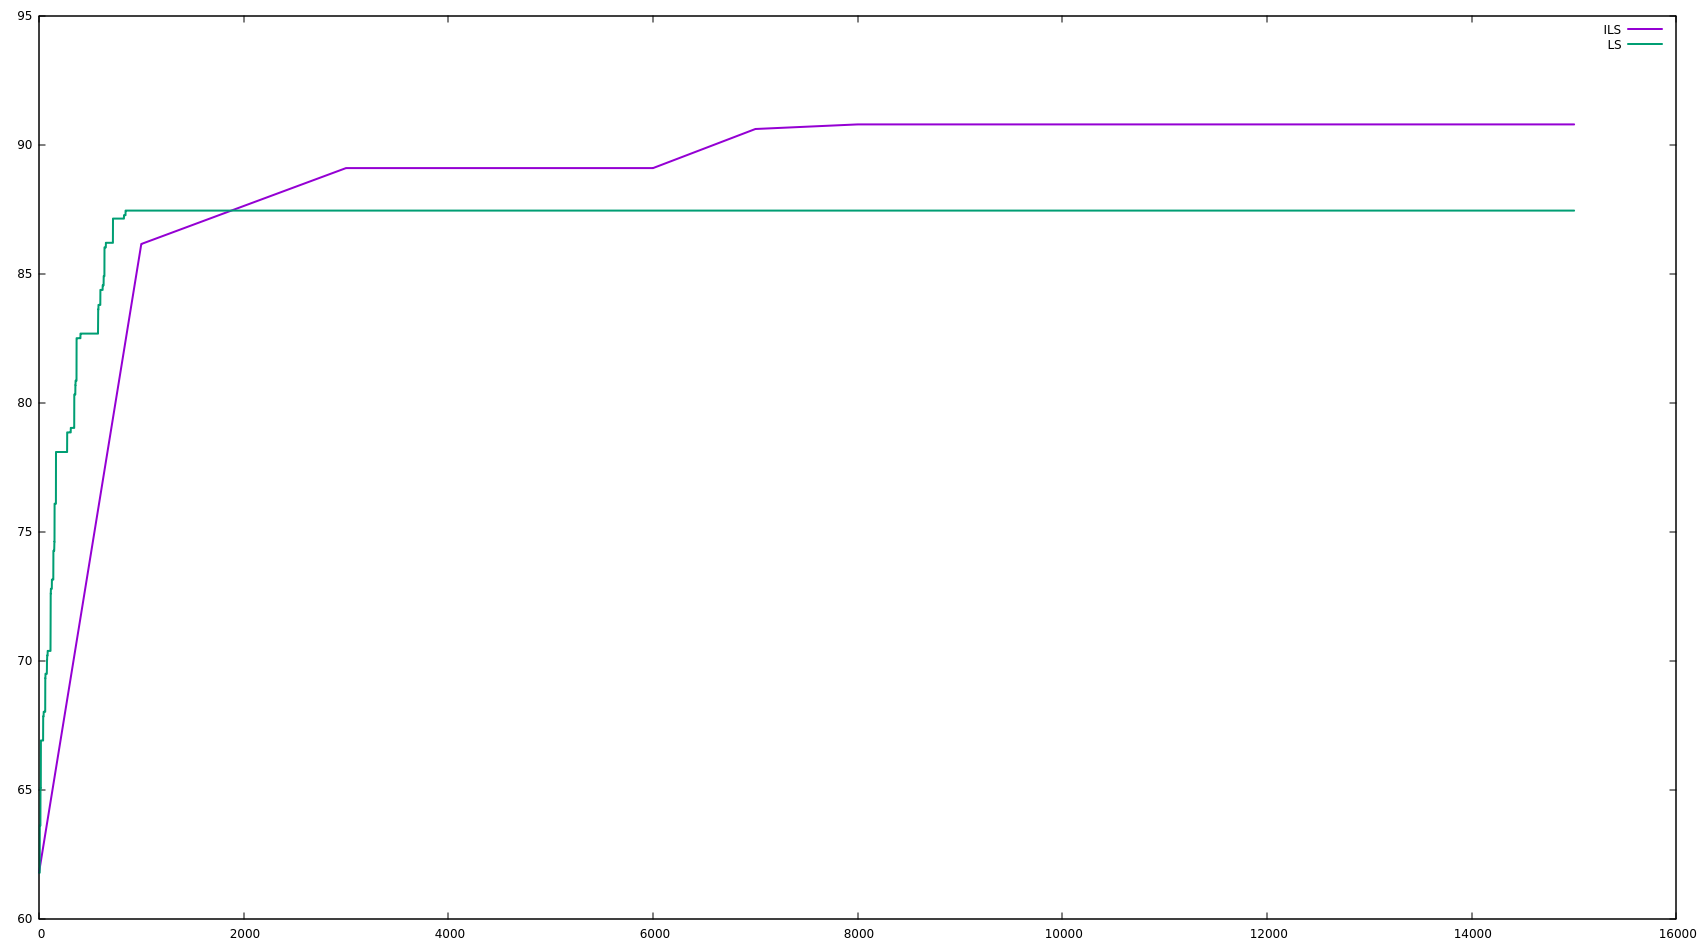
\includegraphics[width=.9\textwidth]{img/ILS-LS.png}
	\caption{Comparación en una ejecución concreta de los algoritmos de BL e ILS en \textit{ionosphere}.}
\end{figure}

Pasamos ya a analizar los algoritmos de \textbf{evolución diferencial}. Lo primero que observamos es que la versión aleatoria \textbf{proporciona los mejores resultados obtenidos hasta el momento con todos los algoritmos}, y en algunos casos con bastante diferencia. Las tasas de reducción obtenidas superan incluso a las obtenidas por los algoritmos genéticos, con un tiempo de ejecución no mucho mayor. Al tener una gran componente aleatoria en la recombinación, conseguimos escapar con facilidad de óptimos locales y seguir aumentando el valor de la función objetivo.\\

Sin embargo, cuando analizamos la versión \textit{current-to-best}, que podríamos pensar que sería incluso mejor, vemos que los resultados dejan bastante que desear. Esta segunda versión queda por debajo de muchos algoritmos, e incluso llega a ser superada por la búsqueda local. Esto puede deberse a que introducimos una gran presión selectiva en el esquema de reemplazamiento, obteniendo una convergencia prematura hacia un óptimo local. Este efecto podemos observarlo en la gráfica de la página siguiente.\\

\begin{figure}[ht!]
    \centering
    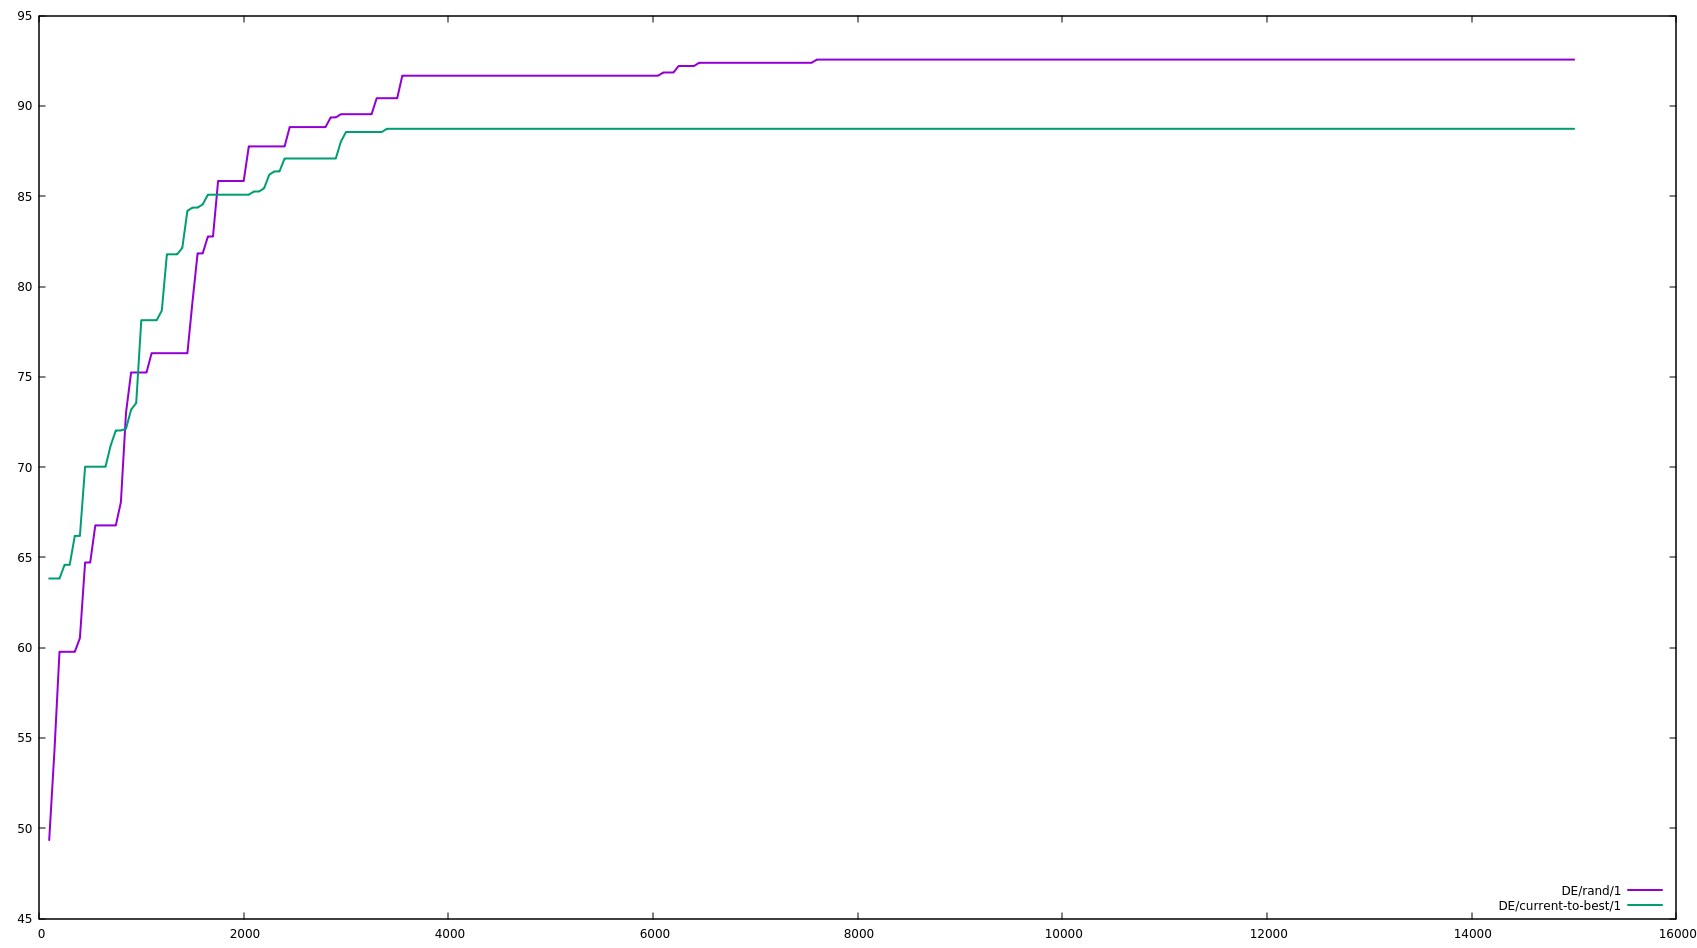
\includegraphics[width=.9\textwidth]{img/DE.png}
	\caption{Comparación en una ejecución concreta de los algoritmos de DE en \textit{ionosphere}.}
\end{figure}

\begin{figure}[ht!]
    \centering
    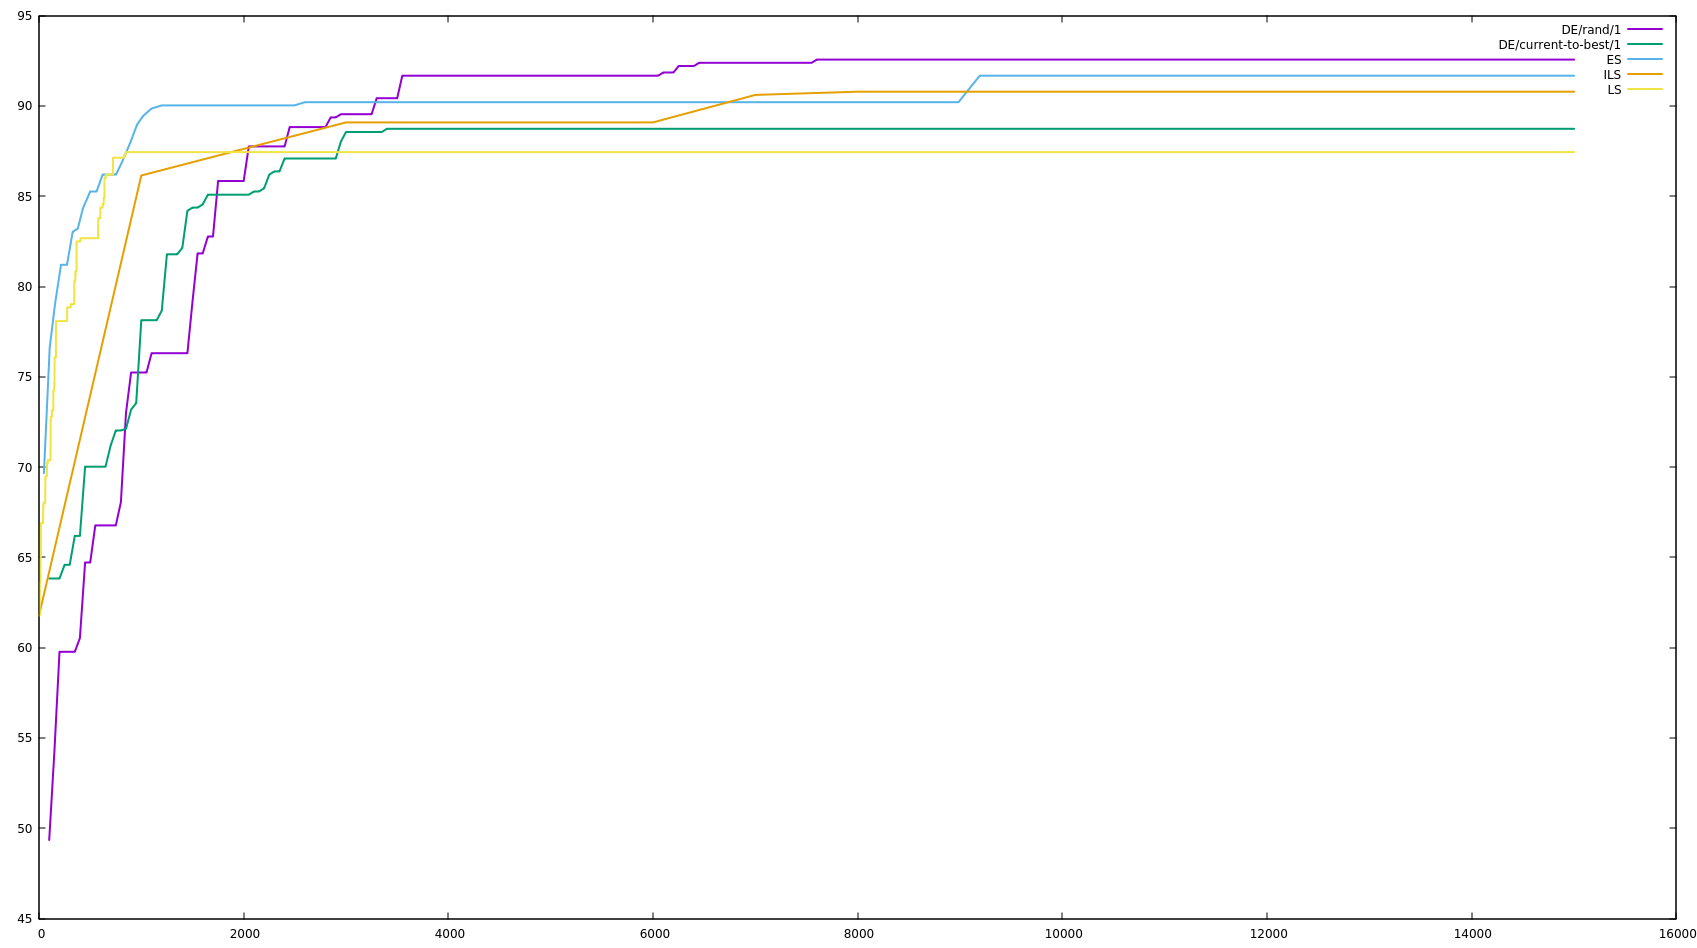
\includegraphics[width=0.7\textwidth]{img/todos.png}
	\caption{Comparación en una ejecución concreta de todos los algoritmos en \textit{ionosphere}.}
\end{figure}

Por último, podemos observar que en general los algoritmos implementados en esta práctica son mejores que los implementados en la práctica 1, y bastante competitivos (y en muchos casos mejores) con los algoritmos genéticos y meméticos de la práctica 2. Notamos que los algoritmos de búsqueda basados en trayectorias no necesitan estructuras de datos auxiliares como los basados en poblaciones, y el código es bastante sencillo e intuitivo. \\

El tiempo de ejecución para todos los algoritmos nuevos es similiar, y también parecido al de los algoritmos genéticos y meméticos. Aunque superan en tiempo de ejecución a la búsqueda local, parece que en este caso esta inversión extra sí merece la pena, pues los resultados obtenidos son mejores. El objetivo de los algoritmos implementados era intentar corregir los defectos que planteaba la búsqueda local, en particular el estancamiento prematuro en óptimos locales, y podemos concluir que el efecto conseguido es el deseado.\\

Tras implementar todos los algoritmos a lo largo del curso, la conclusión a la que podemos llegar es que es complicado encontrar una metaheurística que se adapte perfectamente a todos los conjuntos de datos y casos del problema, y que consiga también un balance entre la exploración y explotación de soluciones para obtener finalmente una lo suficientemente buena.

\end{document}
